% Source: Fukuda (2026), Supplementary Ch. 13 "Optimization: Theorem of the
% Maximum" (pp. 465-484): Def. 13.1-13.9, Remarks 13.1-13.4, Examples 13.1-13.7,
% Lemmas 13.1-13.5, Propositions 13.1-13.9, Corollary 13.1, Theorem 13.1 (Berge's
% Theorem of the Maximum, p. 476), Theorem 13.2 (Kakutani, p. 478); and Sec. 8.2
% (Theorem 8.1, Brouwer, p. 270; Corollary 8.4, p. 271).
% The material is not on the Gerzensee slides; it is the supplementary chapter
% that supplies the existence arguments the slides' equilibrium and dynamic
% programming applications presuppose (Optimization slides 21, Dynamic
% Programming slides 12-24).
% External references actually cited in this chapter: Aliprantis-Border
% (2006), Ok (2007), Rockafellar (1970).
% Danskin's theorem is added to make precise the differentiability claim about
% value functions that the Berge section states informally.

\chapter{Correspondences, the Maximum Theorem and Fixed Points}
\label{ch:maximum}

\section{Why Set-Valued Maps}\label{sec:corr-motivation}

The optimisation of \autoref{ch:optimization} produced a maximiser and treated it
as a point. Two features of economic models make that treatment inadequate.

The maximiser need not be unique. Consumer demand is single-valued only when
preferences are strictly convex; with linear indifference curves the consumer is
indifferent over a whole face of the budget set, and the demand \emph{set} moves
discontinuously as relative prices cross the ratio at which the linear
indifference curves are parallel to the budget line. In game theory the best
response to a mixed strategy is generically a vertex of the simplex but is a
whole face whenever the player is indifferent, and indifference is what
characterises equilibrium in mixed strategies. Nothing can be said about the
existence of equilibrium if the objects being compared are required to be
single-valued.

The feasible set itself moves with the parameters. In the consumer's problem the
budget set depends on prices and income; in a dynamic programme the set of
feasible continuations depends on the current state. Asking whether the value of
the problem varies continuously with the parameters is therefore a question about
the joint behaviour of a function and a moving domain, and it cannot be posed
until the movement of the domain has been given a topology.

This chapter supplies both. It defines continuity for set-valued maps, proves
Berge's theorem that the value function of a parametrised programme is continuous
and the maximiser correspondence upper hemicontinuous, and states the two
fixed-point theorems --- Brouwer's for functions and Kakutani's for
correspondences --- on which the existence of Walrasian and Nash equilibrium
rests. \autoref{thm:banach-fixed-point} gave a fixed-point theorem of a different
kind, and \autoref{prop:fixed-point-comparison} recorded the trade: contraction
buys uniqueness and an algorithm at the price of a Lipschitz hypothesis, whereas
Brouwer and Kakutani buy existence alone, from compactness and convexity, with no
uniqueness and no constructive procedure.

\section{Correspondences}\label{sec:corr-basic}

\begin{definition}[Correspondence]\label{def:correspondence}
	A \dfnas{correspondence}{correspondence} $\varphi\colon X\rightrightarrows Y$
	from a set $X$ into a set $Y$ is a function $\varphi\colon X\to\pow(Y)$ into the
	power set of $Y$; with each $x\in X$ it associates a subset $\varphi(x)$ of $Y$.
	Its \dfnas{graph of a correspondence}{graph} is
	\[
		\gph\varphi\eqdef\{(x,y)\in X\times Y : y\in\varphi(x)\}\subseteq X\times Y,
	\]
	and $\varphi$ is recovered from it by
	$\varphi(x)=\{y\in Y : (x,y)\in\gph\varphi\}$.
	\nidx{correspondence}{$\varphi\colon X\rightrightarrows Y$, correspondence}
	\nidx{graph2}{$\gph\varphi$, graph of a correspondence}
\end{definition}

The definition permits $\varphi(x)=\emptyset$; $\varphi$ is
\dfnas{non-empty-valued correspondence}{non-empty-valued} if
$\varphi(x)\neq\emptyset$ for every $x$. A function $f\colon X\to Y$ is the
single-valued correspondence $x\mapsto\{f(x)\}$, so every statement below
specialises to a statement about functions. Identifying $\varphi$ with $\gph\varphi$ also identifies it
with a binary relation from $X$ to $Y$ in the sense of
\autoref{ch:sets}, which is the reason the graph, rather than the map into
$\pow(Y)$, is the object one topologises.

\begin{definition}[Value restrictions]\label{def:corr-values}
	Let $X,Y$ be topological spaces. A correspondence
	$\varphi\colon X\rightrightarrows Y$ is \dfn{open-valued},
	\dfn{closed-valued}, \dfn{compact-valued} or \dfn{convex-valued} if
	$\varphi(x)$ is respectively open, closed, compact or convex in $Y$ for every
	$x\in X$ (convexity requiring $Y$ to be a vector space).
\end{definition}

\begin{eg}[Budget and demand correspondences]\label{eg:budget-correspondence}
	Define $B\colon\R^{2}_{++}\times\R_+\rightrightarrows\R^2_+$ by
	\begin{equation}\label{eq:budget-correspondence}
		B(p,m)\eqdef\{x\in\R^2_+ : \ip{p}{x}\leq m\} .
	\end{equation}
	By \autoref{eg:budget-compact} the budget set is compact when $p\gg0$, and it is
	convex as the intersection of $\R^2_+$ with a half-space, so $B$ is
	compact-valued, closed-valued and convex-valued. The associated \dfnas{demand correspondence}{demand
		correspondence}
	\begin{equation}\label{eq:demand-correspondence}
		D(p,m)\eqdef\argmax_{x\in B(p,m)}\ u(x)
	\end{equation}
	is the leading example of an \emph{argmax} correspondence, which associates with
	each parameter the set of maximisers. It is non-empty-valued whenever $u$ is
	continuous, by \autoref{cor:weierstrass-continuous}, and it is single-valued
	whenever $u$ is strictly quasiconcave, by
	\autoref{prop:strict-quasi-unique}; without strict quasiconcavity it need be
	neither.
\end{eg}

\begin{eg}[A correspondence with a closed graph]\label{eg:band}
	$\varphi\colon\R\rightrightarrows\R$, $\varphi(x)=[x-1,x+1]$, has graph
	$\gph\varphi=\{(x,y) : \abs{y-x}\leq1\}$, a closed band about the diagonal. It is
	compact-valued and convex-valued.
\end{eg}

\subsection{Two inverses}

A function has one inverse image; a correspondence has two, according to whether
the whole value or merely part of it is required to land in the target set. The
distinction is the source of the two distinct notions of continuity.

\begin{definition}[Upper and lower inverse]\label{def:corr-inverse}
	Let $\varphi\colon X\rightrightarrows Y$ and $A\subseteq Y$. The \dfnas{upper inverse}{upper
		inverse} (or strong inverse) and \dfnas{lower
		inverse}{lower inverse} (or weak inverse) of $A$ are
	\begin{equation}\label{eq:corr-inverses}
		\varphi^{u}(A)\eqdef\{x\in X : \varphi(x)\subseteq A\},
		\qquad
		\varphi^{\ell}(A)\eqdef\{x\in X : \varphi(x)\cap A\neq\emptyset\} .
	\end{equation}
\end{definition}

If $\varphi$ is single-valued, $\varphi^{u}(A)=f^{-1}(A)=\varphi^{\ell}(A)$, so
the two notions coincide precisely on functions.

\begin{proposition}[Calculus of the two inverses]\label{prop:corr-inverse-algebra}
	Let $\varphi\colon X\rightrightarrows Y$ and let $A,B\subseteq Y$ and
	$(A_i)_{i\in I}$ be subsets of $Y$.
	\begin{enumerate}[(i)]
		\item If $\varphi$ is non-empty-valued then
		      $\varphi^{u}(A)\subseteq\varphi^{\ell}(A)$.
		\item $\varphi^{u}(A)=\bigl(\varphi^{\ell}(A^{c})\bigr)^{c}$ and
		      $\varphi^{\ell}(A)=\bigl(\varphi^{u}(A^{c})\bigr)^{c}$.
		\item $\varphi^{u}\bigl(\bigcap_iA_i\bigr)=\bigcap_i\varphi^{u}(A_i)$ and
		      $\varphi^{\ell}\bigl(\bigcup_iA_i\bigr)=\bigcup_i\varphi^{\ell}(A_i)$.
		\item $A\subseteq B$ implies $\varphi^{u}(A)\subseteq\varphi^{u}(B)$ and
		      $\varphi^{\ell}(A)\subseteq\varphi^{\ell}(B)$; consequently
		      $\bigcup_i\varphi^{u}(A_i)\subseteq\varphi^{u}\bigl(\bigcup_iA_i\bigr)$ and
		      $\varphi^{\ell}\bigl(\bigcap_iA_i\bigr)\subseteq\bigcap_i\varphi^{\ell}(A_i)$,
		      both inclusions being strict in general.
	\end{enumerate}
\end{proposition}

\begin{proof}
	(i) If $\varphi(x)\subseteq A$ and $\varphi(x)\neq\emptyset$ then
	$\varphi(x)\cap A=\varphi(x)\neq\emptyset$.

	(ii) $x\notin\varphi^{\ell}(A^{c})$ says $\varphi(x)\cap A^{c}=\emptyset$, that
	is $\varphi(x)\subseteq A$, which is $x\in\varphi^{u}(A)$. The second identity
	is the first applied to $A^{c}$ and complemented.

	(iii) $\varphi(x)\subseteq\bigcap_iA_i$ if and only if
	$\varphi(x)\subseteq A_i$ for every $i$; and
	$\varphi(x)\cap\bigcup_iA_i\neq\emptyset$ if and only if
	$\varphi(x)\cap A_i\neq\emptyset$ for some $i$.

	(iv) Monotonicity is immediate from \eqref{eq:corr-inverses}, and the two
	inclusions follow. For strictness take $X=\{x\}$, $Y=\{1,2\}$,
	$\varphi(x)=\{1,2\}$, $A_1=\{1\}$, $A_2=\{2\}$: then
	$\varphi^{u}(A_1)\cup\varphi^{u}(A_2)=\emptyset$ while
	$\varphi^{u}(A_1\cup A_2)=\{x\}$, and dually
	$\varphi^{\ell}(A_1\cap A_2)=\emptyset$ while
	$\varphi^{\ell}(A_1)\cap\varphi^{\ell}(A_2)=\{x\}$.
\end{proof}

Part (iii) is the reason the two inverses divide the work of
\autoref{prop:image-preimage}, where a single preimage commuted with both unions
and intersections. Set-valuedness breaks that symmetry, and the break is what
forces two continuity concepts rather than one.

\section{Hemicontinuity}\label{sec:hemicontinuity}

\begin{definition}[Upper and lower hemicontinuity]\label{def:hemicontinuity}
	Let $X,Y$ be topological spaces and $\varphi\colon X\rightrightarrows Y$.
	\begin{enumerate}[(i)]
		\item $\varphi$ is \dfnas{upper hemicontinuity}{upper hemicontinuous} at
		      $x\in X$ if for every open $U\supseteq\varphi(x)$ there is an open
		      neighbourhood $V$ of $x$ with $\varphi(z)\subseteq U$ for every $z\in V$.
		\item $\varphi$ is \dfnas{lower hemicontinuity}{lower hemicontinuous} at
		      $x\in X$ if for every open $U$ with $\varphi(x)\cap U\neq\emptyset$ there is
		      an open neighbourhood $V$ of $x$ with $\varphi(z)\cap U\neq\emptyset$ for
		      every $z\in V$.
		\item $\varphi$ is \dfn{continuous} at $x$ if it is both; and $\varphi$ is upper
		      hemicontinuous, lower hemicontinuous or continuous if it is so at every
		      point of $X$.
	\end{enumerate}
\end{definition}

Both conditions compare the values at points \emph{near} $x$ with the value
\emph{at} $x$, and neither restricts $\varphi(x)$ itself. Upper hemicontinuity
says that the nearby values do not stick out: they are contained in any
prescribed open set around $\varphi(x)$ once $z$ is close enough, so no point of
$\varphi(z)$ can stay at a fixed distance from $\varphi(x)$ as $z\to x$. Lower
hemicontinuity says that the nearby values do not leave gaps: they meet every
open set that $\varphi(x)$ meets, so every point of $\varphi(x)$ is approximated
by points of $\varphi(z)$. In the sequential form of
\autoref{thm:uhc-sequential} and \autoref{thm:lhc-sequential} the asymmetry is
plainest: upper hemicontinuity constrains the limits of arbitrary selections
$y_n\in\varphi(x_n)$ to lie in $\varphi(x)$, while lower hemicontinuity requires
each $y\in\varphi(x)$ to be the limit of some such selection. A value set that is
large at $x$ and small nearby therefore satisfies the first and violates the
second, and one that is small at $x$ and large nearby does the reverse, as
\autoref{eg:hemicontinuity-independent} shows. Neither implies the other.

\begin{proposition}[Global characterisations]\label{prop:hemicontinuity-global}
	Let $\varphi\colon X\rightrightarrows Y$ between topological spaces.
	\begin{enumerate}[(i)]
		\item $\varphi$ is upper hemicontinuous if and only if $\varphi^{u}(V)$ is open
		      in $X$ for every open $V\subseteq Y$, if and only if $\varphi^{\ell}(F)$ is
		      closed in $X$ for every closed $F\subseteq Y$.
		\item $\varphi$ is lower hemicontinuous if and only if $\varphi^{\ell}(V)$ is
		      open in $X$ for every open $V\subseteq Y$, if and only if $\varphi^{u}(F)$
		      is closed in $X$ for every closed $F\subseteq Y$.
	\end{enumerate}
	Consequently a single-valued correspondence is upper hemicontinuous if and only
	if it is lower hemicontinuous, if and only if the underlying function is
	continuous.
\end{proposition}

\begin{proof}
	(i) Suppose $\varphi$ is upper hemicontinuous and $V\subseteq Y$ is open. If
	$x\in\varphi^{u}(V)$ then $V$ is an open set containing $\varphi(x)$, so there
	is an open $W\ni x$ with $\varphi(z)\subseteq V$ for all $z\in W$, that is
	$W\subseteq\varphi^{u}(V)$; hence $\varphi^{u}(V)$ is open. Conversely, if
	$\varphi^{u}(V)$ is open for every open $V$ and $U\supseteq\varphi(x)$ is open,
	then $\varphi^{u}(U)$ is an open set containing $x$ and serves as the required
	neighbourhood. The equivalence with the closed-set statement is
	\autoref{prop:corr-inverse-algebra}(ii): $\varphi^{u}(V)$ open for all open $V$
	means $\varphi^{\ell}(V^{c})=\varphi^{u}(V)^{c}$ closed for all such $V$, and
	$V\mapsto V^{c}$ is a bijection between open and closed sets.

	(ii) The same argument with the roles of the two inverses exchanged.

	The final claim follows because for a single-valued $\varphi$ the two inverses
	agree with $f^{-1}$, and \autoref{thm:continuity-preimage} identifies continuity
	of $f$ with openness of $f^{-1}(V)$ for open $V$.
\end{proof}

\begin{eg}[The two notions are independent]\label{eg:hemicontinuity-independent}
	Define $\varphi,\psi,\gamma\colon[0,1]\rightrightarrows[0,1]$ by
	\[
		\varphi(x)=\begin{cases}\{0\}, & x\in[0,1), \\ [0,1], & x=1,\end{cases}
		\qquad
		\psi(x)=\begin{cases}[0,1], & x\in[0,1), \\ \{0\}, & x=1,\end{cases}
		\qquad
		\gamma(x)=[0,1].
	\]
	Then $\varphi$ is upper hemicontinuous everywhere but not lower
	hemicontinuous at $x=1$: the open set $U=(\tfrac12,1]$ meets $\varphi(1)$ but
	misses $\varphi(z)=\{0\}$ for every $z<1$. Symmetrically $\psi$ is lower
	hemicontinuous everywhere but not upper hemicontinuous at $x=1$: the open set
	$U=[0,\tfrac12)$ contains $\psi(1)$ but contains no $\psi(z)$ with $z<1$. The
	constant correspondence $\gamma$ is continuous.

	The two failures are the two ways a jump at $x=1$ can go. For $\varphi$ the
	value at $1$ is larger than every value nearby; nearby values therefore cannot
	stick out of a neighbourhood of $\varphi(1)$, and upper hemicontinuity survives,
	while the part of $\varphi(1)$ away from $0$ is approximated by nothing, and
	lower hemicontinuity fails. For $\psi$ the value at $1$ is smaller than every
	value nearby; every point of $\psi(1)$ is trivially approximated, and lower
	hemicontinuity survives, while the nearby values stick out of any small
	neighbourhood of $\psi(1)=\{0\}$, and upper hemicontinuity fails. The three
	graphs are drawn in \autoref{fig:hemicontinuity}.
\end{eg}

\begin{figure}[htbp]
	\centering
	% Figures/hemicontinuity.tex
% Illustrates Example \ref{eg:hemicontinuity-independent} of Chapter
% \ref{ch:maximum}: the correspondences varphi, psi, gamma on [0,1] showing that
% upper and lower hemicontinuity are logically independent.
% Source: Fukuda (2026), Supplementary Ch. 13, Example 13.4 (p. 470).
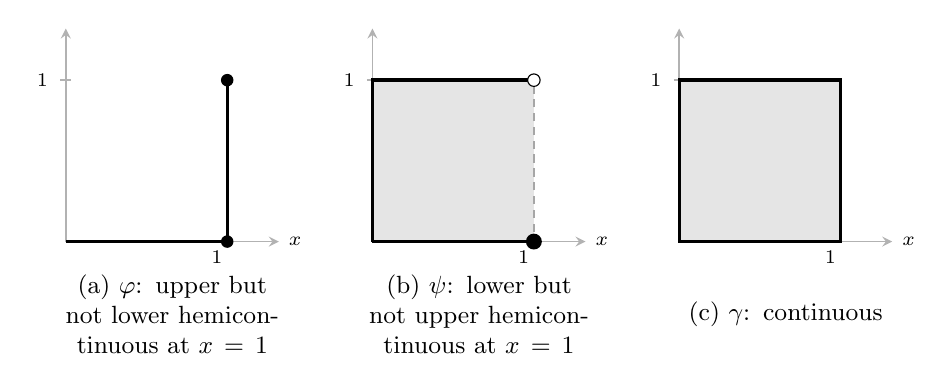
\begin{tikzpicture}[
		scale=2.05,
		>=stealth,
		axisline/.style={->,gray!60,semithick},
		graphline/.style={line width=1.2pt,black},
		excluded/.style={line width=0.7pt,gray!70,densely dashed},
		caption/.style={font=\small,text width=3.15cm,align=center},
	]

	% ---------- phi: uhc but not lhc ----------
	\begin{scope}
		\draw[axisline] (0,0) -- (1.32,0) node[right,black,font=\scriptsize] {$x$};
		\draw[axisline] (0,0) -- (0,1.32);
		\draw[gray!60,semithick] (-0.035,1) -- (0.035,1);
		\draw[gray!60,semithick] (1,-0.035) -- (1,0.035);
		\node[left,font=\scriptsize] at (-0.05,1) {$1$};
		\node[below left,font=\scriptsize,inner sep=1.5pt] at (1,-0.03) {$1$};
		\draw[graphline] (0,0) -- (1,0);
		\draw[graphline] (1,0) -- (1,1);
		\fill (1,1) circle (1.1pt);
		\fill (1,0) circle (1.1pt);
		\node[caption] at (0.66,-0.45) {(a)~$\varphi$: upper but not lower
			hemicontinuous at $x=1$};
	\end{scope}

	% ---------- psi: lhc but not uhc ----------
	\begin{scope}[shift={(1.9,0)}]
		\fill[black!10] (0,0) rectangle (1,1);
		\draw[axisline] (0,0) -- (1.32,0) node[right,black,font=\scriptsize] {$x$};
		\draw[axisline] (0,0) -- (0,1.32);
		\draw[gray!60,semithick] (-0.035,1) -- (0.035,1);
		\node[left,font=\scriptsize] at (-0.05,1) {$1$};
		\node[below left,font=\scriptsize,inner sep=1.5pt] at (1,-0.03) {$1$};
		\draw[graphline] (0,0) -- (0,1) -- (1,1);
		\draw[graphline] (0,0) -- (1,0);
		\draw[excluded] (1,0.06) -- (1,1);
		\draw[fill=white] (1,1) circle (1.1pt);
		\fill (1,0) circle (1.4pt);
		\node[caption] at (0.66,-0.45) {(b)~$\psi$: lower but not upper
			hemicontinuous at $x=1$};
	\end{scope}

	% ---------- gamma: continuous ----------
	\begin{scope}[shift={(3.8,0)}]
		\fill[black!10] (0,0) rectangle (1,1);
		\draw[axisline] (0,0) -- (1.32,0) node[right,black,font=\scriptsize] {$x$};
		\draw[axisline] (0,0) -- (0,1.32);
		\draw[gray!60,semithick] (-0.035,1) -- (0.035,1);
		\node[left,font=\scriptsize] at (-0.05,1) {$1$};
		\node[below left,font=\scriptsize,inner sep=1.5pt] at (1,-0.03) {$1$};
		\draw[graphline] (0,0) rectangle (1,1);
		\node[caption] at (0.66,-0.45) {(c)~$\gamma$: continuous};
	\end{scope}

\end{tikzpicture}

	\caption[Upper and lower hemicontinuity are independent]{The graphs of the
		three correspondences of \autoref{eg:hemicontinuity-independent}. Shading
		marks the values; a dashed edge is not part of the graph. In (a) the value
		at $x=1$ is larger than the neighbouring values, which is compatible with
		upper hemicontinuity and destroys lower hemicontinuity; in (b) it is
		smaller, and the two verdicts are exchanged. Both properties compare
		$\varphi(z)$ for $z$ near $1$ with $\varphi(1)$, not the reverse.}
	\label{fig:hemicontinuity}
\end{figure}

\begin{proposition}[Compactness is preserved]\label{prop:corr-compact-image}
	Let $\varphi\colon X\rightrightarrows Y$ be compact-valued and upper
	hemicontinuous, and let $A\subseteq X$ be compact. Then
	$\varphi(A)\eqdef\bigcup_{x\in A}\varphi(x)$ is compact in $Y$.
\end{proposition}

\begin{proof}
	Let $\mathcal{V}$ be an open cover of $\varphi(A)$. Fix $x\in A$. The compact set
	$\varphi(x)$ is covered by finitely many members of $\mathcal{V}$; let $U_x$ be
	their union, an open set containing $\varphi(x)$. Upper hemicontinuity supplies
	an open $W_x\ni x$ with $\varphi(z)\subseteq U_x$ for $z\in W_x$. The family
	$(W_x)_{x\in A}$ covers the compact set $A$, so finitely many
	$W_{x_1},\dots,W_{x_k}$ suffice, and then
	$\varphi(A)\subseteq\bigcup_{i=1}^{k}U_{x_i}$, a union of finitely many finite
	subfamilies of $\mathcal{V}$.
\end{proof}

This generalises the statement that a continuous image of a compact set is
compact (\autoref{prop:continuous-compact}), and both hypotheses are needed: the
upper hemicontinuous but non-compact-valued $\varphi(x)=\R$ has non-compact
image, and the compact-valued but not upper hemicontinuous $\psi$ of
\autoref{eg:hemicontinuity-independent} would fail if $[0,1]$ were replaced by an
unbounded set.

\subsection{Closed graphs}

\begin{definition}[Closed graph]\label{def:closed-graph}
	A correspondence $\varphi\colon X\rightrightarrows Y$ between topological spaces
	\dfnas{closed graph}{has a closed graph} if $\gph\varphi$ is closed in
	$X\times Y$ with the product topology.
\end{definition}

\begin{theorem}[Closed graph theorem]\label{thm:closed-graph}
	Let $X$ be a metric space and $Y$ a compact metric space. A correspondence
	$\varphi\colon X\rightrightarrows Y$ has a closed graph if and only if it is
	upper hemicontinuous and closed-valued.
\end{theorem}

\begin{proof}
	($\Leftarrow$) A closed subset of a compact metric space is compact, so a
	closed-valued $\varphi$ into $Y$ is compact-valued. Let
	$(x,y)\notin\gph\varphi$. Since $\varphi(x)$ is compact and $y\notin\varphi(x)$,
	the number $\varepsilon\eqdef\dist(y,\varphi(x))$ is strictly positive, and
	$U\eqdef\bigcup_{z\in\varphi(x)}\ball{\varepsilon/2}{z}$ is an open set
	containing $\varphi(x)$ and disjoint from $\ball{\varepsilon/2}{y}$. Upper
	hemicontinuity gives an open $W\ni x$ with $\varphi(w)\subseteq U$ for
	$w\in W$, so $\bigl(W\times\ball{\varepsilon/2}{y}\bigr)\cap\gph\varphi=\emptyset$
	and $(\gph\varphi)^{c}$ is open.

	($\Rightarrow$) A closed graph gives closed values, since
	$\varphi(x)=\{y : (x,y)\in\gph\varphi\}$ is the slice of a closed set. Suppose
	$\varphi$ fails to be upper hemicontinuous at some $x$: there is an open
	$V\supseteq\varphi(x)$ such that every neighbourhood of $x$ contains a point
	whose value is not contained in $V$. Taking the neighbourhoods
	$\ball{1/n}{x}$ produces $x_n\to x$ and $y_n\in\varphi(x_n)\setminus V$. Since
	$Y$ is compact, \autoref{thm:compact-seq-compact} gives a subsequence
	$y_{n_k}\to y$, and $y\in V^{c}$ because $V^{c}$ is closed, so
	$y\notin\varphi(x)$. Then $(x_{n_k},y_{n_k})\in\gph\varphi$ converges to
	$(x,y)\notin\gph\varphi$, and by \autoref{thm:closed-sequential} the graph is
	not closed.
\end{proof}

\begin{remark}[Where compactness of $Y$ is used]\label{rem:closed-graph-compact}
	Without compactness of $Y$ a closed graph does not give upper hemicontinuity.
	Take $X=Y=\R$ and $\varphi(x)=\{1/x\}$ for $x\neq0$, $\varphi(0)=\{0\}$. The
	graph is the hyperbola together with the origin, which is closed in $\R^2$, but
	$\varphi$ is not upper hemicontinuous at $0$: the open set
	$(-1,1)\supseteq\varphi(0)$ contains no $\varphi(z)$ with $z$ small. Economic
	models in which quantities are unbounded require the closed-graph criterion to
	be supplemented by a compactness or boundedness argument before upper
	hemicontinuity may be inferred.
\end{remark}

\subsection{Sequential criteria}

In finite-dimensional applications the definitions are almost always verified
through sequences.

\begin{theorem}[Sequential criterion for upper hemicontinuity]\label{thm:uhc-sequential}
	Let $X\subseteq\R^{k}$ and $Y\subseteq\R^{d}$ and let
	$\varphi\colon X\rightrightarrows Y$ be compact-valued. Then $\varphi$ is upper
	hemicontinuous at $x\in X$ if and only if for every sequence
	$(x_n,y_n)\in\gph\varphi$ with $x_n\to x$ the sequence $(y_n)$ has a subsequence
	converging to a point of $\varphi(x)$.
\end{theorem}

\begin{proof}
	($\Rightarrow$) Let $x_n\to x$ with $y_n\in\varphi(x_n)$. Since $\varphi(x)$ is
	compact it is bounded, so it is contained in some open ball $B$; upper
	hemicontinuity gives a neighbourhood $W$ of $x$ with $\varphi(z)\subseteq B$
	for $z\in W$, and $x_n\in W$ for $n\geq n_0$, whence $y_n\in B$ for such $n$ and
	$(y_n)$ is bounded. By \autoref{thm:bolzano-weierstrass} a subsequence
	$y_{n_k}\to y$ exists. Suppose $y\notin\varphi(x)$. As $\varphi(x)$ is closed
	and non-empty, $\varepsilon\eqdef\dist(y,\varphi(x))>0$, and the open set
	$U\eqdef\bigcup_{z\in\varphi(x)}\ball{\varepsilon/2}{z}$ contains $\varphi(x)$
	but not $y$; indeed $\dist(y,U)\geq\varepsilon/2$. Upper hemicontinuity gives
	$n_1$ with $y_n\in\varphi(x_n)\subseteq U$ for $n\geq n_1$, so
	$y=\lim_ky_{n_k}$ lies in $\closure{U}$, contradicting
	$\dist(y,U)\geq\varepsilon/2$. Hence $y\in\varphi(x)$.

	($\Leftarrow$) Suppose $\varphi$ is not upper hemicontinuous at $x$: there is an
	open $V\supseteq\varphi(x)$ such that for every $n$ some
	$x_n\in\ball{1/n}{x}$ has $\varphi(x_n)\not\subseteq V$. Pick
	$y_n\in\varphi(x_n)\cap V^{c}$. Then $x_n\to x$, and any convergent subsequence
	of $(y_n)$ has its limit in the closed set $V^{c}$, hence outside
	$\varphi(x)\subseteq V$. So no subsequence converges into $\varphi(x)$.
\end{proof}

\begin{theorem}[Sequential criterion for lower hemicontinuity]\label{thm:lhc-sequential}
	Let $X\subseteq\R^{k}$, $Y\subseteq\R^{d}$ and
	$\varphi\colon X\rightrightarrows Y$. Then $\varphi$ is lower hemicontinuous at
	$x$ if and only if for every sequence $x_n\to x$ in $X$ and every
	$y\in\varphi(x)$ there exist $y_n\in\varphi(x_n)$ with $y_n\to y$.
\end{theorem}

\begin{proof}
	($\Rightarrow$) Let $x_n\to x$ and $y\in\varphi(x)$. For each $k\in\N$ the open
	ball $\ball{1/k}{y}$ meets $\varphi(x)$, so lower hemicontinuity gives a
	neighbourhood $U_k$ of $x$ with $\varphi(z)\cap\ball{1/k}{y}\neq\emptyset$ for
	$z\in U_k$. Choose $n_1<n_2<\cdots$ with $x_n\in U_k$ for all $n\geq n_k$. For
	$n_k\leq n<n_{k+1}$ pick $y_n\in\varphi(x_n)\cap\ball{1/k}{y}$, and for
	$n<n_1$ pick $y_n\in\varphi(x_n)$ arbitrarily. Then
	$\norm{y_n-y}<1/k$ once $n\geq n_k$, so $y_n\to y$.

	($\Leftarrow$) Suppose $\varphi$ is not lower hemicontinuous at $x$: there is an
	open $V$ with $\varphi(x)\cap V\neq\emptyset$ such that every neighbourhood of
	$x$ contains a point $z$ with $\varphi(z)\cap V=\emptyset$. Taking
	$\ball{1/n}{x}$ produces $x_n\to x$ with $\varphi(x_n)\cap V=\emptyset$. Fix
	$y\in\varphi(x)\cap V$. Any $y_n\in\varphi(x_n)$ lies in the closed set
	$V^{c}$, so no such sequence can converge to $y\in V$.
\end{proof}

\begin{remark}[The asymmetry of the two criteria]\label{rem:hemicontinuity-asymmetry}
	The two criteria are not mirror images, and the difference is exactly the
	difference between the two inverses. Upper hemicontinuity asks that limits of
	\emph{arbitrary} selections stay inside the value at the limit; it is a
	statement about the graph and, with compact values, is equivalent to closedness
	of the graph by \autoref{thm:closed-graph}. Lower hemicontinuity asks that
	\emph{every} point of the value at the limit be approachable by a selection; it
	is a statement about the existence of continuous selections and has no
	closed-graph reformulation. In economic terms: upper hemicontinuity rules out
	the sudden appearance of new optima, lower hemicontinuity rules out the sudden
	disappearance of existing ones.
\end{remark}

\begin{corollary}[Closed sub-correspondences]\label{cor:closed-subcorrespondence}
	Let $\varphi,\psi\colon X\rightrightarrows Y$ between subsets of finite-dimensional
	Euclidean spaces with $\psi(x)\subseteq\varphi(x)$ for all $x$. If $\varphi$ is
	compact-valued and upper hemicontinuous and $\gph\psi$ is closed, then $\psi$ is
	upper hemicontinuous and compact-valued.
\end{corollary}

\begin{proof}
	$\psi(x)$ is a closed subset of the compact set $\varphi(x)$, hence compact. Let
	$(x_n,y_n)\in\gph\psi$ with $x_n\to x$. Then $(x_n,y_n)\in\gph\varphi$, so by
	\autoref{thm:uhc-sequential} a subsequence $y_{n_k}\to y\in\varphi(x)$. Since
	$(x_{n_k},y_{n_k})\to(x,y)$ and $\gph\psi$ is closed, $(x,y)\in\gph\psi$, that
	is $y\in\psi(x)$. Apply \autoref{thm:uhc-sequential} again.
\end{proof}

\subsection{Operations}

\begin{proposition}[Composition, union, intersection, product]\label{prop:corr-operations}
	Let $X,Y,Z$ be topological spaces.
	\begin{enumerate}[(i)]
		\item For $\varphi\colon X\rightrightarrows Y$ and $\psi\colon Y\rightrightarrows Z$
		      define $(\psi\circ\varphi)(x)\eqdef\bigcup_{y\in\varphi(x)}\psi(y)$. Then
		      $(\psi\circ\varphi)^{u}(A)=\varphi^{u}(\psi^{u}(A))$ and
		      $(\psi\circ\varphi)^{\ell}(A)=\varphi^{\ell}(\psi^{\ell}(A))$, and the
		      composition inherits upper, respectively lower, hemicontinuity from both
		      factors.
		\item A union of lower hemicontinuous correspondences is lower
		      hemicontinuous; a union of two upper hemicontinuous correspondences is
		      upper hemicontinuous.
		\item If $\varphi$ has a closed graph and $\psi$ is upper hemicontinuous and
		      compact-valued, then $\varphi\cap\psi$ is upper hemicontinuous.
		\item A product of upper hemicontinuous compact-valued correspondences is upper
		      hemicontinuous and compact-valued; a product of lower hemicontinuous
		      correspondences is lower hemicontinuous.
	\end{enumerate}
\end{proposition}

\begin{proof}
	(i) For the upper inverse,
	$x\in(\psi\circ\varphi)^{u}(A)$ says $\psi(y)\subseteq A$ for every
	$y\in\varphi(x)$, that is $\varphi(x)\subseteq\psi^{u}(A)$; the lower inverse is
	analogous with ``some'' in place of ``every''. Hemicontinuity then follows from
	\autoref{prop:hemicontinuity-global}: openness of $\psi^{u}(V)$ and of
	$\varphi^{u}$ of an open set compose.

	(ii) For unions, $\bigl(\bigcup_i\varphi_i\bigr)^{\ell}(V)
		=\bigcup_i\varphi_i^{\ell}(V)$ is open when each summand is; for two upper
	hemicontinuous correspondences,
	$(\varphi\cup\psi)^{u}(V)=\varphi^{u}(V)\cap\psi^{u}(V)$ is a finite
	intersection of open sets.

	(iii) Let $V\subseteq Y$ be open with $(\varphi\cap\psi)(x)\subseteq V$, and put
	$K\eqdef\psi(x)\setminus V$, a compact set. If $K=\emptyset$ take
	$N\eqdef\psi^{u}(V)$. Otherwise each $y\in K$ lies outside $\varphi(x)$, so
	$(x,y)\notin\gph\varphi$, and closedness of the graph supplies open
	$U_y\ni x$ and $W_y\ni y$ with $(U_y\times W_y)\cap\gph\varphi=\emptyset$.
	Finitely many $W_{y_1},\dots,W_{y_r}$ cover $K$; set $W\eqdef\bigcup_iW_{y_i}$
	and $N\eqdef\psi^{u}(V\cup W)\cap\bigcap_{i}U_{y_i}$. Since
	$\psi(x)\subseteq V\cup W$, upper hemicontinuity of $\psi$ makes $N$ an open
	neighbourhood of $x$. For $z\in N$ we have $\psi(z)\subseteq V\cup W$ and
	$\varphi(z)\cap W=\emptyset$, hence $(\varphi\cap\psi)(z)\subseteq V$.

	(iv) See \textcite[Thm.~17.28]{aliprantis2006infinite}; the compact-valued case
	in a finite product follows from \autoref{thm:uhc-sequential} applied
	coordinatewise together with \autoref{prop:coordinatewise}.
\end{proof}

\section{Economic Application: Continuity of the Budget Correspondence}
\label{sec:corr-budget}

\begin{proposition}\label{prop:budget-continuous}
	Let $B\colon\R^{n}_{++}\times\R_{++}\rightrightarrows\R^{n}_{+}$ be the budget
	correspondence \eqref{eq:budget-correspondence}. Then $B$ is non-empty-valued,
	compact-valued, convex-valued and continuous.
\end{proposition}

\begin{proof}
	Non-emptiness, compactness and convexity are \autoref{eg:budget-correspondence}.

	\emph{Upper hemicontinuity.} Let $(p_k,m_k)\to(p,m)$ in
	$\R^{n}_{++}\times\R_{++}$ and $x_k\in B(p_k,m_k)$. Since $p\gg0$, there are
	$\underline{p}>0$ and $\bar m<\infty$ with $p_k\geq\underline{p}\one$ and
	$m_k\leq\bar m$ for large $k$, so
	$\norm{x_k}_1\leq\bar m/\underline{p}$ and $(x_k)$ is bounded. By
	\autoref{thm:bolzano-weierstrass} a subsequence converges, say
	$x_{k_j}\to x\geq0$, and passing to the limit in
	$\ip{p_{k_j}}{x_{k_j}}\leq m_{k_j}$ gives $\ip{p}{x}\leq m$, so
	$x\in B(p,m)$. Apply \autoref{thm:uhc-sequential}.

	\emph{Lower hemicontinuity.} Let $(p_k,m_k)\to(p,m)$ and
	$x\in B(p,m)$. If $\ip{p}{x}<m$, then $\ip{p_k}{x}<m_k$ for large $k$ and the
	constant sequence $x_k\eqdef x$ works for those $k$; for the finitely many
	remaining indices take $x_k\eqdef0$. If instead $\ip{p}{x}=m$, set
	\[
		\lambda_k\eqdef\min\Bigl\{1,\ \frac{m_k}{\ip{p_k}{x}}\Bigr\},
		\qquad x_k\eqdef\lambda_kx .
	\]
	Then $x_k\in\R^n_+$ and $\ip{p_k}{x_k}\leq m_k$, so $x_k\in B(p_k,m_k)$; and
	$\ip{p_k}{x}\to\ip{p}{x}=m>0$, so $\lambda_k\to\min\{1,m/m\}=1$ and
	$x_k\to x$. Apply \autoref{thm:lhc-sequential}.
\end{proof}

\begin{eg}[The two boundaries of $\R^n_{++}\times\R_{++}$]
	\label{eg:budget-failures}
	\autoref{prop:budget-continuous} is stated on
	$\R^{n}_{++}\times\R_{++}$. The two boundaries behave differently.

	\emph{Zero wealth is harmless.} The conclusion extends to $m=0$. Upper
	hemicontinuity: the boundedness argument of the proof needs only
	$p\gg0$ and $m_k\leq\bar m$, and the limit $x$ of a convergent subsequence
	satisfies $\ip{p}{x}\leq0$, hence $x=0\in B(p,0)$. Lower hemicontinuity:
	$B(p,0)=\{0\}$ and $0\in B(p_k,m_k)$ for every $k$, so the constant sequence
	$x_k\eqdef0$ suffices. So $B$ is continuous on $\R^n_{++}\times\R_+$, and the
	restriction $m>0$ in \autoref{prop:budget-continuous} is a convenience of the
	proof rather than a boundary of the result.

	\emph{Zero prices are not.} Take $n=2$, $p^{k}=(1,1/k)\to p=(1,0)$ and
	$m=1$. Then $B(p^{k},1)$ is the triangle with vertices $(0,0)$, $(1,0)$,
	$(0,k)$, while $B\bigl((1,0),1\bigr)=\{x\in\R^{2}_{+} : x_1\leq1\}$ is closed
	and unbounded, hence not compact. Compact-valuedness therefore fails, and with
	it both \autoref{thm:uhc-sequential}, whose statement presupposes compact
	values, and the hypotheses of Berge's theorem
	(\autoref{thm:berge-maximum}). This is a loss of the tools, not by itself a
	proof that upper hemicontinuity fails; what does fail, and is the substantive
	point, is existence: a strictly increasing $u$ has no maximiser on the
	unbounded set $B\bigl((1,0),1\bigr)$, so demand is undefined at a zero price.
	General-equilibrium existence proofs respond either by bounding consumption
	sets artificially or by working on the interior of the price simplex and
	handling the boundary separately.

	\emph{Where lower hemicontinuity genuinely fails.} The budget correspondence on
	$\R^n_+$ is lower hemicontinuous because $0$ is always available and always
	cheapest. Replace the consumption set by
	$X\eqdef\{x\in\R^2_+ : x_1\geq1\}$, a subsistence requirement, and set
	$B_X(p,m)\eqdef\{x\in X : \ip{p}{x}\leq m\}$. At $p=(1,1)$ and $m=1$ one has
	$B_X(p,1)=\{(1,0)\}$, whereas $B_X(p,1-1/k)=\emptyset$ for every $k$, since
	$x_1\geq1$ and $x_2\geq0$ force $\ip{p}{x}\geq1$. No selection converges to
	$(1,0)$, so $B_X$ is not lower hemicontinuous at $(p,1)$. The failure is
	exactly the absence of a \dfnas{cheaper point}{cheaper point}: some $x\in X$
	with $\ip{p}{x}<m$. That condition, and not positivity of wealth, is what
	lower hemicontinuity of a budget correspondence rests on.
\end{eg}

\section{Berge's Theorem of the Maximum}\label{sec:berge}

Recall from \autoref{def:semicontinuity} that $m\colon X\to\R$ is lower
semicontinuous if $\{x : m(x)>\alpha\}$ is open for every $\alpha\in\R$, and
upper semicontinuous if $-m$ is lower semicontinuous. The maximum theorem is
proved by establishing the two halves separately, each from one half of the
continuity of the constraint correspondence.

\begin{lemma}[Lower semicontinuity of the value]\label{lem:berge-lsc}
	Let $\varphi\colon X\rightrightarrows Y$ be lower hemicontinuous and let
	$f\colon\gph\varphi\to\R$ be lower semicontinuous. Then
	$m(x)\eqdef\sup_{y\in\varphi(x)}f(x,y)$, with $m(x)=-\infty$ when
	$\varphi(x)=\emptyset$, is lower semicontinuous.
\end{lemma}

\begin{proof}
	Fix $\alpha\in\R$ and $x_0$ with $m(x_0)>\alpha$. Then $f(x_0,y_0)>\alpha$ for
	some $y_0\in\varphi(x_0)$, so $\varphi(x_0)\neq\emptyset$. The set
	$W\eqdef\{(x,y)\in\gph\varphi : f(x,y)>\alpha\}$ is open in $\gph\varphi$ by
	lower semicontinuity of $f$ and contains $(x_0,y_0)$, so there are open
	$U\ni x_0$ in $X$ and $V\ni y_0$ in $Y$ with
	$(U\times V)\cap\gph\varphi\subseteq W$. Put
	$N\eqdef U\cap\varphi^{\ell}(V)$, which is open by
	\autoref{prop:hemicontinuity-global}(ii) and contains $x_0$ because
	$y_0\in\varphi(x_0)\cap V$. For $x\in N$ pick $y\in\varphi(x)\cap V$; then
	$(x,y)\in(U\times V)\cap\gph\varphi\subseteq W$, so $f(x,y)>\alpha$ and
	$m(x)>\alpha$. Hence $\{m>\alpha\}$ is open.
\end{proof}

\begin{lemma}[Upper semicontinuity of the value]\label{lem:berge-usc}
	Let $\varphi\colon X\rightrightarrows Y$ be upper hemicontinuous, non-empty- and
	compact-valued, and let $f\colon\gph\varphi\to\R$ be upper semicontinuous. Then
	$m(x)\eqdef\max_{y\in\varphi(x)}f(x,y)$ is well defined and upper
	semicontinuous.
\end{lemma}

\begin{proof}
	For fixed $x$ the function $f(x,\cdot)$ is upper semicontinuous on the
	non-empty compact set $\varphi(x)$, so \autoref{thm:weierstrass} gives the
	maximum. Fix $\alpha\in\R$ and $x_0$ with $m(x_0)<\alpha$, and put
	$W\eqdef\{(x,y)\in\gph\varphi : f(x,y)<\alpha\}$, open in $\gph\varphi$ and
	containing $\{x_0\}\times\varphi(x_0)$. For each $y\in\varphi(x_0)$ choose open
	$U_y\ni x_0$ and $V_y\ni y$ with $(U_y\times V_y)\cap\gph\varphi\subseteq W$.
	Compactness of $\varphi(x_0)$ gives $y_1,\dots,y_r$ with
	$\varphi(x_0)\subseteq V\eqdef\bigcup_{i}V_{y_i}$; set
	$U\eqdef\bigcap_{i}U_{y_i}$ and $N\eqdef U\cap\varphi^{u}(V)$, open by
	\autoref{prop:hemicontinuity-global}(i) and containing $x_0$. For $x\in N$ and
	$y\in\varphi(x)$ we have $(x,y)\in(U\times V)\cap\gph\varphi\subseteq W$, so
	$f(x,y)<\alpha$ and therefore $m(x)<\alpha$.
\end{proof}

\begin{theorem}[Berge's theorem of the maximum]\label{thm:berge-maximum}
	Let $X,Y$ be topological spaces, let
	$\varphi\colon X\rightrightarrows Y$ be continuous with non-empty compact
	values, and let $f\colon\gph\varphi\to\R$ be continuous. Define the
	\dfnas{value function}{value function} and the \dfnas{argmax correspondence}{argmax
		correspondence}
	\begin{equation}\label{eq:berge-objects}
		m(x)\eqdef\max_{y\in\varphi(x)}f(x,y),
		\qquad
		\mu(x)\eqdef\{y\in\varphi(x) : f(x,y)=m(x)\} .
	\end{equation}
	Then
	\begin{enumerate}[(i)]
		\item $m$ is continuous on $X$;
		\item $\mu$ is non-empty- and compact-valued; and
		\item $\mu$ is upper hemicontinuous.
	\end{enumerate}
\end{theorem}

\begin{proof}
	(i) $f$ is both upper and lower semicontinuous and $\varphi$ is both upper and
	lower hemicontinuous, so \autoref{lem:berge-lsc} and \autoref{lem:berge-usc}
	make $m$ both lower and upper semicontinuous, hence continuous by
	\autoref{cor:semicontinuity-continuity}.

	(ii) Fix $x$. The map $y\mapsto(x,y)$ is continuous from $\varphi(x)$ into
	$\gph\varphi$, so $f(x,\cdot)$ is continuous on the non-empty compact set
	$\varphi(x)$ and attains its maximum there by \autoref{thm:weierstrass}; thus
	$\mu(x)\neq\emptyset$. Moreover $\mu(x)=\{y\in\varphi(x) : f(x,y)\geq m(x)\}$
	is closed in $\varphi(x)$, hence compact.

	(iii) Fix $x_0\in X$ and an open $U\subseteq Y$ with $\mu(x_0)\subseteq U$. Put
	$K\eqdef\varphi(x_0)\setminus U$, a closed subset of the compact set
	$\varphi(x_0)$ and therefore compact. If $K=\emptyset$, then
	$\varphi(x_0)\subseteq U$ and upper hemicontinuity of $\varphi$ supplies an open
	$N\ni x_0$ with $\mu(z)\subseteq\varphi(z)\subseteq U$ for $z\in N$.

	Suppose $K\neq\emptyset$. Every $y\in K$ lies in $\varphi(x_0)$ but not in
	$\mu(x_0)$, so $f(x_0,y)<m(x_0)$; since $f(x_0,\cdot)$ is continuous on the
	compact set $K$ it attains a maximum there, and hence there is
	$\varepsilon>0$ with
	\begin{equation}\label{eq:berge-gap}
		f(x_0,y)<m(x_0)-2\varepsilon\qquad\text{for all }y\in K .
	\end{equation}
	The set $W\eqdef\{(x,y)\in\gph\varphi : f(x,y)<m(x)-\varepsilon\}$ is open in
	$\gph\varphi$, because $f$ is continuous on $\gph\varphi$ and $m$ is continuous
	on $X$ by (i), and \eqref{eq:berge-gap} puts $\{x_0\}\times K$ inside $W$. For
	each $y\in K$ choose open $U_y\ni x_0$ in $X$ and $V_y\ni y$ in $Y$ with
	$(U_y\times V_y)\cap\gph\varphi\subseteq W$. Compactness of $K$ gives
	$y_1,\dots,y_r$ with $K\subseteq V\eqdef\bigcup_{i\leq r}V_{y_i}$; set
	$N_1\eqdef\bigcap_{i\leq r}U_{y_i}$, an open neighbourhood of $x_0$, and note
	that $(N_1\times V)\cap\gph\varphi\subseteq W$.

	Since $\varphi(x_0)\subseteq U\cup V$ and $U\cup V$ is open, upper
	hemicontinuity of $\varphi$ supplies an open $N_2\ni x_0$ with
	$\varphi(z)\subseteq U\cup V$ for $z\in N_2$. Let $z\in N_1\cap N_2$ and
	$y\in\mu(z)$. Then $y\in\varphi(z)\subseteq U\cup V$. Were $y\in V$, then
	$(z,y)\in(N_1\times V)\cap\gph\varphi\subseteq W$ would give
	$f(z,y)<m(z)-\varepsilon$, contradicting $f(z,y)=m(z)$. Hence $y\in U$, so
	$\mu(z)\subseteq U$ for every $z\in N_1\cap N_2$.
\end{proof}

The argument is purely topological: no metric, no sequences and no separation
axiom on $Y$ enters, so the theorem holds as stated for arbitrary topological
spaces. In $\R^n$ the conclusion can also be reached through
\autoref{cor:closed-subcorrespondence}, since $\gph\mu$ is then closed, but that
route needs the sequential criteria and is available only in the metric setting.

\begin{remark}[$\mu$ is not lower hemicontinuous]\label{rem:berge-not-lhc}
	Upper hemicontinuity is the strongest conclusion available. Let $X=[0,1]$,
	$Y=[1,2]$, $\varphi\equiv Y$ and $f(x,y)=y^{x}$. Then
	$\mu(x)=\{2\}$ for $x>0$ and $\mu(0)=Y$, since $f(0,\cdot)\equiv1$ is constant.
	The correspondence $\mu$ is upper hemicontinuous at $0$, as the theorem
	asserts, and is not lower hemicontinuous there: every $y\in[1,2)$ belongs to
	$\mu(0)$ and is approached by no selection from $\mu(x)=\{2\}$. Ties in the
	objective produce large optimal sets that collapse under an arbitrarily small
	perturbation, and no hypothesis of the theorem prevents this. In economics the
	phenomenon is the discontinuous collapse of demand when an indifference curve
	is tangent to a whole segment of the budget line.
\end{remark}

\begin{eg}[Every hypothesis is used]\label{eg:berge-failure}
	Let $X=Y=[0,1]$, $f(x,y)=y$, and
	\[
		\varphi(x)=\begin{cases}[0,1], & x=0, \\ \{0\}, & x>0.\end{cases}
	\]
	Then $\varphi$ is upper hemicontinuous and compact-valued but not lower
	hemicontinuous at $0$. Consequently $m(0)=1$ and $m(x)=0$ for $x>0$, so $m$ is
	not continuous but merely upper semicontinuous, as
	\autoref{lem:berge-usc} predicts; and $\mu(0)=\{1\}$, $\mu(x)=\{0\}$ for
	$x>0$, so $\mu$ is not upper hemicontinuous. Losing lower hemicontinuity of
	the constraint correspondence loses both conclusions at once.
\end{eg}

\begin{corollary}[Continuity of Marshallian demand]\label{cor:demand-uhc}
	Let $u\colon\R^{n}_{+}\to\R$ be continuous. Then the indirect utility function
	$v(p,m)=\max_{x\in B(p,m)}u(x)$ is continuous on
	$\R^{n}_{++}\times\R_{++}$ and the demand correspondence $D$ of
	\eqref{eq:demand-correspondence} is non-empty- and compact-valued and upper
	hemicontinuous there. If in addition $u$ is strictly quasiconcave, $D$ is
	single-valued and the demand function is continuous.
\end{corollary}

\begin{proof}
	\autoref{prop:budget-continuous} and \autoref{thm:berge-maximum} give the first
	two claims, with $f(x,y)\eqdef u(y)$ as the objective. If $u$ is strictly
	quasiconcave, \autoref{prop:strict-quasi-unique} makes $D$ single-valued, and by
	\autoref{prop:hemicontinuity-global} a single-valued upper hemicontinuous
	correspondence is a continuous function.
\end{proof}

The corollary is the theoretical warrant for the comparative statics performed
throughout demand theory. Without it, an expression such as
$\partial x^{\ast}/\partial p$ could not be assumed even to exist, and the
observation of \autoref{rem:comparative-statics-ift} --- that the implicit
function theorem delivers differentiability from a non-singular bordered Hessian
--- would have nothing to be applied to. \autoref{cor:demand-uhc} also shows what
is available without any differentiability at all: continuity of $v$ and upper
hemicontinuity of $D$ come from compactness and continuity alone.

\begin{proposition}[Concavity of the value function]\label{prop:value-concave}
	Let $f\colon\R^{n}\times\R^{k}\to\R$ be concave and suppose
	$f^{\ast}(\alpha)\eqdef\max_{x\in\R^{n}}f(x,\alpha)$ exists for every
	$\alpha\in\R^{k}$. Then $f^{\ast}$ is concave.
\end{proposition}

\begin{proof}
	Fix $\alpha,\alpha'\in\R^{k}$ and $\lambda\in[0,1]$, and choose maximisers
	$x^{\ast}(\alpha),x^{\ast}(\alpha')$. Then
	\begin{align*}
		f^{\ast}\bigl((1-\lambda)\alpha+\lambda\alpha'\bigr)
		 & \geq f\bigl((1-\lambda)x^{\ast}(\alpha)+\lambda x^{\ast}(\alpha'),\,
		(1-\lambda)\alpha+\lambda\alpha'\bigr)                                  \\
		 & \geq(1-\lambda)f\bigl(x^{\ast}(\alpha),\alpha\bigr)
		+\lambda f\bigl(x^{\ast}(\alpha'),\alpha'\bigr)
		=(1-\lambda)f^{\ast}(\alpha)+\lambda f^{\ast}(\alpha'),
	\end{align*}
	the first inequality because the displayed point is feasible and the second by
	concavity of $f$ on $\R^{n}\times\R^{k}$.
\end{proof}

Maximisation over an unconstrained variable therefore preserves concavity. This
is what makes the value function of a concave dynamic programme concave, and hence
--- by \autoref{prop:convex-continuous} --- continuous on the interior of its
domain.

Differentiability is a separate matter, and it does not follow from uniqueness of
the maximiser. Consider
\[
	V(\alpha)\eqdef\max\{x\in\R : x\leq\alpha,\ x\leq1\}=\min\{\alpha,1\}.
\]
The objective is linear, the constraints are affine, the maximiser
$x^\ast(\alpha)=\min\{\alpha,1\}$ is unique for every $\alpha$, and $V$ is
concave; yet $V$ is not differentiable at $\alpha=1$, where the binding
constraint changes. Concavity delivers a non-empty superdifferential at every
interior point and differentiability exactly where that superdifferential is a
singleton, which is a condition on the whole family of supporting affine
functions rather than on the argmax. The theorems that do convert regularity of
the objective into differentiability of the value --- Danskin's theorem, the
envelope theorem \autoref{thm:envelope}, and Benveniste--Scheinkman
(\autoref{thm:benveniste-scheinkman}) --- all assume differentiability of the objective in the
parameter and interiority of the maximiser, and the example above satisfies
neither at $\alpha=1$.

\autoref{thm:danskin} makes the first of these precise and shows exactly how much
regularity of the value function a smooth objective delivers when the maximiser
is not unique.

\begin{theorem}[Danskin]\label{thm:danskin}
	Let $X\subseteq\R^{n}$ be open, $U$ a non-empty compact metric space, and
	$\varphi\colon X\times U\to\R$ continuous with the partial gradient
	$\nabla_{x}\varphi$ existing and continuous on $X\times U$. Put
	\[
		V(x)\eqdef\max_{u\in U}\varphi(x,u),
		\qquad M(x)\eqdef\argmax_{u\in U}\varphi(x,u).
	\]
	Then $V$ is locally Lipschitz on $X$, $M(x)$ is non-empty and compact, and for
	every $x\in X$ and $d\in\R^{n}$ the one-sided directional derivative exists and
	\begin{equation}\label{eq:danskin}
		V'(x;d)\eqdef\lim_{t\downarrow0}\frac{V(x+td)-V(x)}{t}
		=\max_{u\in M(x)}\ \ip{\nabla_{x}\varphi(x,u)}{d} .
	\end{equation}
	If $M(x)=\{u^{\ast}\}$ is a singleton, then $V$ is differentiable at $x$ with
	$\nabla V(x)=\nabla_{x}\varphi(x,u^{\ast})$.
\end{theorem}

\begin{proof}
	Non-emptiness and compactness of $M(x)$, and continuity and upper
	hemicontinuity of $V$ and $M$, are \autoref{thm:berge-maximum} applied to the
	constant correspondence $\Gamma\equiv U$.

	\emph{Local Lipschitz property.} Let $K\subseteq X$ be compact and convex with
	$x\in\Int K$, and put $L\eqdef\max_{K\times U}\norm{\nabla_{x}\varphi}$, finite
	by \autoref{cor:weierstrass-continuous} on the compact $K\times U$. For
	$y,z\in K$,
	\[
		\abs{V(y)-V(z)}\leq\max_{u\in U}\abs{\varphi(y,u)-\varphi(z,u)}\leq L\norm{y-z},
	\]
	the first inequality because $\abs{\max_ua(u)-\max_ub(u)}\leq\max_u\abs{a(u)-b(u)}$
	and the second by the mean value theorem along the segment $[z,y]\subseteq K$.

	\emph{Lower bound in \eqref{eq:danskin}.} Fix $u\in M(x)$. For small $t>0$,
	\[
		V(x+td)-V(x)\geq\varphi(x+td,u)-\varphi(x,u)
		=t\ip{\nabla_{x}\varphi(x,u)}{d}+o(t),
	\]
	so $\liminf_{t\downarrow0}\bigl(V(x+td)-V(x)\bigr)/t
		\geq\ip{\nabla_{x}\varphi(x,u)}{d}$; take the maximum over $u\in M(x)$.

	\emph{Upper bound.} Let $t_k\downarrow0$ realise the limit superior and choose
	$u_k\in M(x+t_kd)$. The mean value theorem applied to
	$s\mapsto\varphi(x+sd,u_k)$ gives $\theta_k\in(0,1)$ with
	\[
		\frac{V(x+t_kd)-V(x)}{t_k}\leq\frac{\varphi(x+t_kd,u_k)-\varphi(x,u_k)}{t_k}
		=\ip{\nabla_{x}\varphi(x+\theta_kt_kd,u_k)}{d}.
	\]
	By compactness of $U$, pass to a subsequence with $u_k\to\bar u$; upper
	hemicontinuity of $M$ together with \autoref{thm:closed-graph} gives
	$\bar u\in M(x)$, and continuity of $\nabla_{x}\varphi$ gives
	$\ip{\nabla_{x}\varphi(x+\theta_kt_kd,u_k)}{d}\to
		\ip{\nabla_{x}\varphi(x,\bar u)}{d}$. Hence the limit superior is at most
	$\max_{u\in M(x)}\ip{\nabla_{x}\varphi(x,u)}{d}$, and \eqref{eq:danskin}
	follows.

	\emph{Differentiability under uniqueness.} Write $g\eqdef\nabla_{x}\varphi(x,u^{\ast})$,
	so that \eqref{eq:danskin} reads $V'(x;d)=\ip{g}{d}$ for every $d$. Suppose $V$
	were not differentiable at $x$ with derivative $g$. Then there are
	$\varepsilon>0$ and $h_k\to0$, $h_k\neq0$, with
	\begin{equation}\label{eq:danskin-contradiction}
		\bigl\lvert V(x+h_k)-V(x)-\ip{g}{h_k}\bigr\rvert\geq\varepsilon\norm{h_k}.
	\end{equation}
	Write $h_k=t_kd_k$ with $t_k=\norm{h_k}\downarrow0$ and $\norm{d_k}=1$; by
	compactness of the unit sphere, pass to a subsequence with $d_k\to d$. The
	local Lipschitz bound gives
	$\abs{V(x+t_kd_k)-V(x+t_kd)}\leq Lt_k\norm{d_k-d}=o(t_k)$, while the
	directional derivative along the fixed direction $d$ gives
	$V(x+t_kd)-V(x)=t_k\ip{g}{d}+o(t_k)$. Therefore
	\[
		V(x+h_k)-V(x)-\ip{g}{h_k}
		=t_k\ip{g}{d-d_k}+o(t_k)=o(t_k),
	\]
	since $d_k\to d$, contradicting \eqref{eq:danskin-contradiction}.
\end{proof}

\begin{remark}[What Danskin adds, and what it does not]\label{rem:danskin-reading}
	Formula \eqref{eq:danskin} holds with no convexity and no uniqueness: the value
	function of a smooth family always has one-sided directional derivatives, and
	they are computed by freezing the maximiser and differentiating the objective.
	What multiplicity of maximisers costs is two-sidedness. Taking $d$ and $-d$ in
	\eqref{eq:danskin},
	\[
		V'(x;d)+V'(x;-d)=\max_{u\in M(x)}\ip{\nabla_{x}\varphi(x,u)}{d}
		-\min_{u\in M(x)}\ip{\nabla_{x}\varphi(x,u)}{d}\geq0,
	\]
	with equality for every $d$ if and only if $\nabla_{x}\varphi(x,\cdot)$ is
	constant on $M(x)$. A kink in the value function is therefore not caused by
	multiplicity of the maximiser as such, but by disagreement among the maximisers
	about the marginal effect of the parameter. In the example $V(\alpha)=\min\{\alpha,1\}$
	above the maximiser is unique at every $\alpha$, and the kink at $\alpha=1$ comes
	instead from the failure of the constraint set to be described by a fixed compact
	$U$ independent of the parameter, which is the hypothesis Danskin's theorem
	imposes and \autoref{thm:berge-maximum} relaxes.

	When each $\varphi(\cdot,u)$ is convex, $V$ is convex by
	\autoref{prop:convex-function-operations}, and every
	$\nabla_{x}\varphi(x,u)$ with $u\in M(x)$ is a subgradient of $V$ at $x$: for
	any $y$,
	\[
		V(y)\geq\varphi(y,u)\geq\varphi(x,u)+\ip{\nabla_{x}\varphi(x,u)}{y-x}
		=V(x)+\ip{\nabla_{x}\varphi(x,u)}{y-x},
	\]
	using \autoref{thm:concave-gradient} for the middle inequality. Since
	$\partial V(x)$ is closed and convex by \autoref{thm:subgradient-exists}, it
	contains $\conv\{\nabla_{x}\varphi(x,u) : u\in M(x)\}$. Equality of the two sets
	is the identification of $V'(x;\cdot)$ with the support function of
	$\partial V(x)$ and is proved in
	\textcite[Sec.~23]{rockafellar1970convex}; it is not used below.
\end{remark}

For constrained problems, concavity of the value function in the parameter needs
the constraint correspondence to have a convex \emph{graph}, not merely convex
values. The budget correspondence \eqref{eq:budget-correspondence} has a convex
graph in $(x,m)$ for fixed $p$, so if $u$ is concave then $v(p,\cdot)$ is concave
in wealth. In prices the graph is not convex, and the conclusion available is
different in kind: $v$ is quasiconvex in $(p,m)$ jointly (\autoref{ex:cvx-2}),
homogeneous of degree zero in $(p,m)$, non-increasing in each price and
non-decreasing in wealth. It need not be convex in $p$. Take $n=1$ and
$u(x)=-x^{-2}$ on $(0,\infty)$, which is strictly increasing and strictly
concave since $u'(x)=2x^{-3}>0$ and $u''(x)=-6x^{-4}<0$. Demand exhausts the
budget, so $x(p,m)=m/p$ and
\[
	v(p,m)=-\Bigl(\frac{p}{m}\Bigr)^{2},
	\qquad
	\frac{\partial^{2}v}{\partial p^{2}}=-\frac{2}{m^{2}}<0,
\]
strictly concave in $p$. It remains quasiconvex, being monotone in a single
variable. Convexity in $p$ does occur --- $u(x)=\log x$ gives
$v(p,m)=\log m-\log p$ with $\partial^{2}v/\partial p^{2}=p^{-2}>0$ --- but it
is a feature of the particular utility function and not a general property.

\section{Fixed-Point Theorems}\label{sec:fixed-points}

\begin{theorem}[Brouwer]\label{thm:brouwer}
	Let $C\subseteq\R^{n}$ be non-empty, compact and convex. Every continuous
	$f\colon C\to C$ has a fixed point.
\end{theorem}

The proof is topological --- it rests on the fact that the $n$-sphere is not a
retract of the closed ball --- and is not reproduced here; see
\textcite[Ch.~E]{ok2007real} for a full treatment and
\textcite[p.~270]{fukuda2026notes} for the statement used in this course. What is
reproduced is the exact role of each hypothesis, since the failures are what one
must check in applications.

\begin{eg}[The three hypotheses of Brouwer]\label{eg:brouwer-failures}
	\emph{Compactness.} $C=\R$ and $f(x)=x+1$: continuous, $C$ convex, no fixed
	point. Closedness alone is not enough, and neither is boundedness alone: on
	$C=(0,1)$ the map $f(x)=x/2$ is continuous with no fixed point.

	\emph{Convexity.} $C=\{x\in\R^{2} : \norm{x}=1\}$, the unit circle, is compact
	but not convex, and the rotation by $\pi$, $f(x)=-x$, is continuous with no
	fixed point.

	\emph{Continuity.} $C=[0,1]$ and $f(x)=1$ for $x<\tfrac12$, $f(x)=0$ for
	$x\geq\tfrac12$: compact convex domain, no fixed point.
\end{eg}

\begin{corollary}[Brouwer on the simplex]\label{cor:brouwer-simplex}
	Let $\Delta^{n-1}\eqdef\{p\in\R^{n}_{+} : \sum_{i=1}^{n}p_i=1\}$. Every
	continuous $f\colon\Delta^{n-1}\to\Delta^{n-1}$ has a fixed point.
\end{corollary}

\begin{proof}
	$\Delta^{n-1}$ is convex as the intersection of $\R^n_+$ with a hyperplane, and
	compact by \autoref{thm:heine-borel}, being closed and contained in the unit
	ball of $\norm{\cdot}_1$.
\end{proof}

\begin{theorem}[Kakutani]\label{thm:kakutani}
	Let $X\subseteq\R^{n}$ be non-empty, compact and convex, and let
	$\varphi\colon X\rightrightarrows X$ be non-empty-valued, convex-valued and have
	a closed graph. Then $\varphi$ has a \dfnas{fixed point of a
		correspondence}{fixed point}: some $x\in X$ with $x\in\varphi(x)$.
\end{theorem}

By \autoref{thm:closed-graph} the closed-graph hypothesis is, on a compact $X$,
the same as requiring $\varphi$ upper hemicontinuous with closed values.
Kakutani's theorem contains Brouwer's: a continuous function is a single-valued
correspondence with convex values and, by
\autoref{prop:hemicontinuity-global} and \autoref{thm:closed-graph}, a closed
graph. The statement is \textcite[Thm.~13.2, p.~478]{fukuda2026notes}; the proof,
which approximates $\varphi$ by continuous functions on successively finer
simplicial subdivisions and applies Brouwer to each, is in
\textcite[Ch.~17]{aliprantis2006infinite}.

\begin{eg}[The four hypotheses of Kakutani]\label{eg:kakutani-failures}
	\emph{Compactness.} $X=\R$, $\varphi(x)=\{x+1\}$.

	\emph{Convexity of $X$.} $X$ the unit circle, $\varphi(x)=\{-x\}$.

	\emph{Convex values.} $X=[0,1]$ and $\varphi(x)=\{0,1\}\setminus\{x\}$ for
	$x\in\{0,1\}$, $\varphi(x)=\{0,1\}$ otherwise. This has a closed graph and
	compact values, but $x\in\varphi(x)$ never holds. A cleaner instance is
	$X=[0,1]$ with $\varphi(x)=\{1\}$ for $x<\tfrac12$, $\varphi(1/2)=\{0,1\}$ and
	$\varphi(x)=\{0\}$ for $x>\tfrac12$: the graph is closed, the values are compact
	and non-empty, and only convexity at $x=\tfrac12$ fails, which is where
	a fixed point would have to be.

	\emph{Closed graph.} $X=[0,1]$ with $\varphi(x)=\{1\}$ for $x<\tfrac12$ and
	$\varphi(x)=\{0\}$ for $x\geq\tfrac12$: convex-valued, non-empty-valued, no
	fixed point, and the graph is not closed at $x=\tfrac12$.
\end{eg}

\section{Economic Application: Existence of Nash Equilibrium}
\label{sec:corr-nash}

\paragraph{Environment.} A finite game has players indexed by
$i\in\{1,\dots,I\}$, finite
action sets $A_i$, and payoffs $u_i\colon\prod_jA_j\to\R$. A mixed strategy for
player $i$ is an element $\sigma_i$ of the simplex $\Delta(A_i)$ over $A_i$.
Write $\Sigma\eqdef\prod_i\Delta(A_i)$ and extend $u_i$ to $\Sigma$ by
expectation,
\begin{equation}\label{eq:mixed-payoff}
	u_i(\sigma)\eqdef\sum_{a\in\prod_jA_j}\Bigl(\prod_{j=1}^{I}\sigma_j(a_j)\Bigr)u_i(a).
\end{equation}
A \dfnas{Nash equilibrium}{Nash equilibrium} is $\sigma^{\ast}\in\Sigma$ with
$u_i(\sigma^{\ast})\geq u_i(\sigma_i,\sigma^{\ast}_{-i})$ for every $i$ and every
$\sigma_i\in\Delta(A_i)$.

\begin{theorem}[Nash]\label{thm:nash-existence}
	Every finite game has a Nash equilibrium in mixed strategies.
\end{theorem}

\begin{proof}
	Define the best-response correspondence
	$\beta_i\colon\Sigma\rightrightarrows\Delta(A_i)$ by
	$\beta_i(\sigma)\eqdef\argmax_{\sigma_i\in\Delta(A_i)}u_i(\sigma_i,\sigma_{-i})$
	and set $\beta\eqdef\prod_i\beta_i\colon\Sigma\rightrightarrows\Sigma$. A fixed
	point of $\beta$ is precisely a Nash equilibrium, by the definition of
	$\beta_i$. The hypotheses of \autoref{thm:kakutani} are verified in turn.

	\emph{$\Sigma$ is non-empty, compact and convex.} Each $\Delta(A_i)$ is a
	simplex, compact and convex by \autoref{cor:brouwer-simplex}'s argument, and a
	finite product of compact convex sets is compact by
	\autoref{prop:compact-stability} and convex by
	\autoref{prop:convex-operations}.

	\emph{$\beta$ is non-empty-valued.} $u_i(\cdot,\sigma_{-i})$ is a polynomial,
	hence continuous, on the compact set $\Delta(A_i)$, so
	\autoref{cor:weierstrass-continuous} applies.

	\emph{$\beta$ is convex-valued.} By \eqref{eq:mixed-payoff}, $u_i$ is
	\emph{affine} in $\sigma_i$ for fixed $\sigma_{-i}$. The set of maximisers of an
	affine function on a convex set is convex: if
	$u_i(\sigma_i,\sigma_{-i})=u_i(\sigma_i',\sigma_{-i})=\max$ then affinity gives
	the same value at every convex combination. A product of convex sets is convex.

	\emph{$\beta$ has a closed graph.} The constraint correspondence
	$\sigma\mapsto\Delta(A_i)$ is constant, hence continuous with non-empty compact
	values, and $u_i$ is continuous on $\Sigma\times\Delta(A_i)$; so
	\autoref{thm:berge-maximum}(iii) makes $\beta_i$ upper hemicontinuous with
	compact values, and \autoref{thm:closed-graph} converts this into a closed graph
	on the compact space $\Sigma$. Closed graphs are preserved by finite products.

	\autoref{thm:kakutani} now supplies $\sigma^{\ast}\in\beta(\sigma^{\ast})$.
\end{proof}

Two features of the argument deserve emphasis. Convex-valuedness rests entirely
on the \emph{linearity} of expected utility in own mixed strategy; it is what
mixing is for, and it is why an equilibrium in pure strategies need not exist
while one in mixed strategies always does. And upper hemicontinuity of the best
response is an instance of \autoref{thm:berge-maximum} in the degenerate case of
a constant constraint correspondence, so the maximum theorem is doing the work
even where no constraint moves.

\section{Economic Application: Existence of Walrasian Equilibrium}
\label{sec:corr-walras}

\paragraph{Environment.} There are $n$ goods and a price vector $p$ normalised to
lie in $\Delta^{n-1}$. Let $Z\colon\Delta^{n-1}\to\R^{n}$ denote aggregate excess
demand: $Z_i(p)$ is the quantity of good $i$ demanded in aggregate, net of the
aggregate endowment, at prices $p$.

\begin{assumption}[Excess demand]\label{ass:excess-demand}
	$Z$ is continuous on $\Delta^{n-1}$ and satisfies \dfnas{Walras' law}{Walras'
		law} $\ip{p}{Z(p)}=0$ for every $p\in\Delta^{n-1}$.
\end{assumption}

Walras' law is the aggregate budget identity: each consumer spends exactly their
wealth, so the value of aggregate excess demand is zero at every price vector,
whether or not markets clear. Continuity of $Z$ is not primitive; it is the
conclusion of \autoref{cor:demand-uhc} applied to each consumer, requiring
strictly quasiconcave utility for single-valuedness and interior prices for
compactness of the budget set (\autoref{eg:budget-failures}).

\begin{theorem}[Existence of equilibrium prices]\label{thm:walras-existence}
	Under \autoref{ass:excess-demand} there exists $p^{\ast}\in\Delta^{n-1}$ with
	$Z(p^{\ast})\leq0$; and $Z_i(p^{\ast})<0$ only if $p^{\ast}_i=0$.
\end{theorem}

\begin{proof}
	Define $g\colon\Delta^{n-1}\to\Delta^{n-1}$ by
	\begin{equation}\label{eq:price-adjustment}
		g_i(p)\eqdef\frac{p_i+\max\{0,Z_i(p)\}}{1+\sum_{k=1}^{n}\max\{0,Z_k(p)\}} .
	\end{equation}
	The denominator is at least $1$, the numerators are non-negative and sum to the
	denominator, so $g$ maps $\Delta^{n-1}$ into itself; $g$ is continuous because
	$Z$ is and $t\mapsto\max\{0,t\}$ is. By \autoref{cor:brouwer-simplex} there is
	$p^{\ast}$ with $g(p^{\ast})=p^{\ast}$. Writing
	$S\eqdef\sum_{k}\max\{0,Z_k(p^{\ast})\}$, the fixed-point equation is
	$p^{\ast}_i(1+S)=p^{\ast}_i+\max\{0,Z_i(p^{\ast})\}$, that is
	\begin{equation}\label{eq:walras-fixed-point}
		p^{\ast}_iS=\max\{0,Z_i(p^{\ast})\}\qquad\text{for each }i .
	\end{equation}
	Multiply \eqref{eq:walras-fixed-point} by $Z_i(p^{\ast})$ and sum over $i$:
	\[
		S\underbrace{\ip{p^{\ast}}{Z(p^{\ast})}}_{=0\ \text{(Walras)}}
		=\sum_{i=1}^{n}Z_i(p^{\ast})\max\{0,Z_i(p^{\ast})\}
		=\sum_{i=1}^{n}\bigl(\max\{0,Z_i(p^{\ast})\}\bigr)^{2} .
	\]
	A sum of squares equal to zero forces $\max\{0,Z_i(p^{\ast})\}=0$ for every $i$,
	that is $Z(p^{\ast})\leq0$. Finally, if $Z_i(p^{\ast})<0$ for some $i$ with
	$p^{\ast}_i>0$, then $\ip{p^{\ast}}{Z(p^{\ast})}<0$ because every term is at
	most zero and this one is strictly negative, contradicting Walras' law.
\end{proof}

The map \eqref{eq:price-adjustment} is a normalised \emph{t\^atonnement}: prices
of goods in excess demand are raised in proportion to the excess, prices of the
remaining goods fall through the normalisation. The theorem says the process has
a rest point; it says nothing about whether the process converges to it, and in
general it does not. The last sentence of the statement is free disposal in
equilibrium: a good in strict excess supply must be free.

\begin{remark}[What has and has not been proved]\label{rem:walras-caveats}
	\autoref{thm:walras-existence} is a statement about a function $Z$ that has been
	\emph{assumed} continuous on the whole simplex, boundary included. Deriving that
	hypothesis from preferences and endowments is the substance of the existence
	problem, and it is where the difficulties of \autoref{eg:budget-failures} bite:
	as some $p_i\to0$ the budget set ceases to be compact and, under monotone
	preferences, demand for good $i$ diverges, so $Z$ is unbounded near the
	boundary. The standard resolutions --- truncating consumption sets to a large
	compact box and showing the truncation does not bind, or replacing $Z$ by a
	correspondence and invoking \autoref{thm:kakutani} in the form of the
	Gale--Nikaid\^o--Debreu lemma --- are treated in
	\textcite[Ch.~17]{aliprantis2006infinite}. What the argument above establishes
	cleanly is that once continuity and Walras' law are available, existence is a
	one-page consequence of Brouwer's theorem.
\end{remark}

\section{Chapter Summary}\label{sec:corr-summary}

A correspondence is a map into subsets, identified with its graph. Because a
correspondence has two inverse images --- the upper inverse demanding containment
of the whole value, the lower inverse demanding only non-empty intersection ---
there are two continuity notions, both comparing the values near a point with the
value at it. Upper hemicontinuity, equivalent to openness of upper inverses of
open sets and, on compact ranges, to closedness of the graph, keeps the nearby
values inside any prescribed neighbourhood of the value at the point; lower
hemicontinuity requires the nearby values to reach every part of it. In finite
dimensions both are checked by sequences: upper hemicontinuity says every
selection along a convergent sequence of parameters has a subsequence converging
into the limit value, lower hemicontinuity says every point of the limit value is
the limit of some selection.

The budget correspondence is continuous with compact convex values at strictly
positive prices, wealth zero included, and loses compact-valuedness when a price
is zero; lower hemicontinuity is what fails when the consumption set admits no
point cheaper than the wealth level.
Berge's theorem of the maximum then yields, for a continuous objective on the
graph of a continuous compact-valued constraint correspondence, a continuous
value function and an upper hemicontinuous compact-valued argmax; lower
hemicontinuity of the argmax is false in general, and the counterexample is
ties in the objective. Applied to the consumer, this gives continuity of indirect
utility and upper hemicontinuity of Marshallian demand, single-valued and
continuous under strict quasiconcavity. Maximising out a variable preserves
concavity of the objective in the remaining parameters, but not
differentiability, which requires the separate hypotheses of the envelope and
Benveniste--Scheinkman theorems.

Existence of equilibrium comes from fixed points. Brouwer's theorem gives a fixed
point of a continuous self-map of a non-empty compact convex set; Kakutani's
extends this to correspondences that are non-empty- and convex-valued with a
closed graph. Kakutani applied to the best-response correspondence gives Nash
equilibrium in mixed strategies, convex-valuedness being the linearity of
expected utility in own strategy. Brouwer applied to a normalised t\^atonnement
map gives Walrasian equilibrium prices from continuity of excess demand and
Walras' law. Neither theorem gives uniqueness, and neither gives an algorithm ---
in contrast to \autoref{thm:banach-fixed-point}, which gives both at the cost of
a contraction hypothesis.

\begin{exercise}\label{ex:corr-1}
	Prove \autoref{prop:hemicontinuity-global} in the pointwise form: $\varphi$ is
	upper hemicontinuous at $x$ if and only if $\varphi^{u}(U)$ is a neighbourhood
	of $x$ for every neighbourhood $U$ of $\varphi(x)$; and dually for lower
	hemicontinuity. Then show directly from the definitions that a correspondence
	is upper hemicontinuous and lower hemicontinuous at $x$ if and only if it is
	continuous there.
\end{exercise}

\begin{exercise}\label{ex:corr-2}
	Let $\varphi\colon X\rightrightarrows Y$ be a correspondence and $A\subseteq X$.
	Prove that $A\subseteq\varphi^{u}(\varphi(A))$, and that if $\varphi$ is
	non-empty-valued then $A\subseteq\varphi^{\ell}(\varphi(A))$. Give an example in
	which both inclusions are strict, and reconcile the result with
	\autoref{prop:image-preimage}.
\end{exercise}

\begin{exercise}\label{ex:corr-3}
	Let $\Gamma\colon S\rightrightarrows S$ be the feasible-continuation
	correspondence of a dynamic programme on a compact state space $S$, assumed
	continuous with non-empty compact values, and let
	$F\colon\gph\Gamma\to\R$ be continuous and $\beta\in(0,1)$. Using
	\autoref{thm:berge-maximum}, show that the Bellman operator
	$(Tv)(s)=\max_{s'\in\Gamma(s)}\{F(s,s')+\beta v(s')\}$ maps
	$\Cspace{S}{\R}$ into itself, and combine this with
	\autoref{prop:C-complete} and \autoref{thm:blackwell} to conclude that the value
	function is the unique continuous fixed point and that the policy
	correspondence is upper hemicontinuous. This is the argument completed in
	\autoref{ch:dynamic}.
\end{exercise}
